
\chapter{到射影空间的映射与线丛的性质}
\label{ch:maps-projective-properties}

\trVariety{} $X$ 上的\trLineBundle{}之所以重要，部分原因在于它们能让我们知道许多关于从 $X$ 到其他\trVariety{}的映射的信息——这是因为它们告知了我们从 $X$ 到\trProjectiveSpace{}的映射（\S15.2）。\trLineBundle{}的「\trAmpleness」这一关键概念，应当看成某种「正性」（positivity）（\S16.2），它将帮助我们了解\trLineBundle{}何时拥有大量\trSection，甚至给出到\trProjectiveSpace{}的映射。\trAmpleness{}的基本事实需要花些功夫才能建立，但此后将威力十足地派上用场。例如，在 \S16.3 中，我们将看到许多对\trCurve{}的应用。


\section{整体生成的拟凝聚层}

我们从一个结果开始，它让我们能够借助\trLineBundle{}来「够着」\trProjectiveScheme{}上的任何\trFiniteType{}的\trQCSheaf。本节通篇，$S_\bullet$ 都将是 $A$ 上一个\trFinitelyGenerated{}的\trGradedRing，在次数 $1$ 处生成。我们将证明下述结果。

\textbf{16.1.1.\ \trhTheorem{}。}\ ——\ \emph{$\Proj S_\bullet$ 上任何\trFiniteType{}的\trQCSheaf{} $\mathscr{F}$ 均能表成如下形式}
\[
\oplus_{\mathrm{finite}}\OO(-\mathfrak{m})\longrightarrow\mathscr{F}\longrightarrow 0.
\]

由于我们能够亲手摆弄这些\trLineBundle{} $\OO(-\mathfrak{m})$，这一结果将让我们对 $\Proj S_\bullet$ 上的\emph{一切}\trCoherentSheaf（特别是\trVectorBundle）都有很强的掌控。作为一个初例，它将使我们得以证明：\trProjective{} $k$-\trScheme{}上每个\trCoherentSheaf{}的\trGlobalSections{}都构成一个\trFiniteDimensional{}的\trVectorSpace（\mbox{推论~18.1.4}）。（这个事实日后将长大为这样一个事实：\trCoherentSheaf{}在\trProper{}态射下的高阶前推也是\trCoh{}的；见\mbox{定理~18.7.1}(d) 与\trGrothendieck{}凝聚定理~18.9.1。）

我们不径直奔向证明，而是拿它作个借口，来介绍一些在更宽泛的场合有用的观念（\emph{\trGlobalGeneration}（global generation）、\emph{无基点性}（base-point-freeness）、\emph{\trAmpleness}（ampleness））以及它们之间的相互关系。但首先我们拿它作借口，来提一条重要的经典结果。

\textbf{16.1.2.}\ \emph{\trHilbert{}\trSyzygy{}定理。}

对 $\mathbb{P}^n_k$ 上任一\trCoherentSheaf{} $\mathscr{F}$，\mbox{定理~16.1.1} 给出了\trSurjectiveMap{} $\phi\colon\oplus_{\mathrm{finite}}\OO(-\mathfrak{m})\to\mathscr{F}\to 0$ 的存在性。这个\trSurjectiveMap{}的\trKernel{}也是\trCoh{}的，于是迭代这一构造，我们便能构造出 $\mathscr{F}$ 的一个由\trLineBundle{}的\trDirectSum{}给出的无穷分解（infinite resolution）：
\[
\cdots\;\oplus_{\mathrm{finite}}\OO(\mathfrak{m}_{2,j})\longrightarrow\oplus_{\mathrm{finite}}\OO(\mathfrak{m}_{1,j})\longrightarrow\oplus_{\mathrm{finite}}\OO(\mathfrak{m}_{0,j})\longrightarrow\mathscr{F}\longrightarrow 0.
\]

\textbf{16.1.3.\ \trHilbert{}\trSyzygy{}定理。}\ ——\ \emph{存在一个有限的分解，其长度至多为 $n+1$。}

这一结果的最初历史，见\mbox{定理~3.6.17} 之后的评述。我们不会用到这条定理，但其证明将在选读的 \S24.4 中给出。

\textbf{16.1.4.\ \trGloballyGenerated\trSheaf。}\quad 设 $X$ 是一个\trScheme，而 $\mathscr{F}$ 是一个 $\OO$-\trModule。本节最重要的定义就是如下这个：称 $\mathscr{F}$ 为\textbf{\trGloballyGenerated}（globally generated）（或\textbf{由\trGlobalSections{}生成}（generated by global sections）），若它容许一个来自 $X$ 上某个\trFreeSheaf{}的\trSurjectiveMap：
\[
\OO^{\oplus I}\twoheadrightarrow\mathscr{F}.
\]
这里 $I$ 是某个\trIndexSet。此处所论的那些\trGlobalSections，便是 $\OO_X^{\oplus I}$ 的各个直和项里对应于 $1$ 的那 $|I|$ 个\trSection{}的像；这些像生成 $\mathscr{F}$ 的各\trStalk。若\trIndexSet{} $I$ 可以取为有限的，我们便说 $\mathscr{F}$ 是\textbf{有限整体生成的}（finitely globally generated）（或\textbf{由有限多个\trGlobalSections{}生成}（generated by a finite number of global sections））。

更多的定义，说得再细致些：我们说 $\mathscr{F}$ \textbf{在点 $p$ 处整体生成}（globally generated at a point $p$）（或有时说\textbf{在 $p$ 处由\trGlobalSections{}生成}（generated by global sections at $p$）），如果我们能找到一个 $\phi\colon\OO^{\oplus I}\to\mathscr{F}$，它在 $p$ 处的\trStalk{}上是\trSurjectiveMap，
\[
\OO_{\mathfrak{p}}^{\oplus I}\overset{\phi_{\mathfrak{p}}}{\twoheadrightarrow}\mathscr{F}_{\mathfrak{p}}.
\]
（说得更精确些，应当是：$\mathscr{F}$ 在 $p$ 处的\trStalk{}由 $\mathscr{F}$ 的\trGlobalSections{}生成。）关键的洞见在于：在 $p$ 处的整体生成，意味着 $p$ 处的每一个\trGerm{}都是诸\trGlobalSections{}的\trGerm{}的一个线性组合（组合系数取在\trLocalRing{} $\OO_{X,p}$ 中）。

注意，若 $\mathscr{F}$ 在\emph{一切}点 $p$ 处都整体生成，则 $\mathscr{F}$ 是\emph{\trGloballyGenerated}。（理由：\mbox{练习~2.4.D} 已证明\trIsomorphism{}可以在\trStalk{}的层面上检验；同一论证的一个更容易的版本表明，\trSurjectiveMap{}性也可以在\trStalk{}的层面上检验。）请注意，我们可以为整个 $X$ 取定单一的\trIndexSet，办法是把各个 $p$ 的诸\trIndexSet{}取并。

\textbf{16.1.A.（容易的练习）}\quad $X$ 上的一个\trInvertibleSheaf{} $\mathscr{L}$ 是\trGloballyGenerated，当且仅当对任意点 $p\in X$，都存在 $\mathscr{L}$ 的一个在 $p$ 处不消失的\trSection；也就是说，$\mathscr{L}$ 是\trBasePointFree{}的（\mbox{定义~15.2.1}）。

\textbf{16.1.B.（容易的练习：现实检验）}\quad 证明：每个\trAffineScheme{}上的每个\trQCSheaf{}都是\trGloballyGenerated。证明：每个\trAffineScheme{}上的每个\trFiniteType{}的\trQCSheaf{}都由有限多个\trGlobalSections{}生成。（两者共用的提示：对任何 $A$-\trModule{} $M$，总有一个从自由 $A$-\trModule{}到 $M$ 的\trSurjectiveMap。）

显然，若 $\mathscr{F}$ 与 $\mathscr{G}$ 都\trGloballyGenerated，则 $\mathscr{F}\oplus\mathscr{G}$ 亦然（对有限整体生成、在点 $p$ 处生成等等情形亦复如是）。对张量积也有类似的道理：

\textbf{16.1.C.（容易的练习：整体生成的$\otimes$整体生成的是整体生成的）}\quad 证明：若\trQCSheaf{} $\mathscr{F}$ 与 $\mathscr{G}$ 在点 $p$ 处整体生成，则 $\mathscr{F}\otimes\mathscr{G}$ 亦然。（若 $\mathscr{F}$ 与 $\mathscr{G}$ 是\trInvertibleSheaf，这正是\mbox{练习~15.2.B}。）

\textbf{16.1.D.（容易但重要的练习）}\quad 设 $\mathscr{F}$ 是 $X$ 上一个\trFiniteType{}的\trQCSheaf。

（a）证明：$\mathscr{F}$ 在点 $p$ 处整体生成，当且仅当「$\mathscr{F}$ 的\trFiber{}在 $p$ 处由\trGlobalSections{}生成」，也就是说，诸\trGlobalSections{}作为一个\trVectorSpace{}张成\trFiber{} $\mathscr{F}_{\mathfrak{p}}/\mathfrak{m}\mathscr{F}_{\mathfrak{p}}$，其中 $\mathfrak{m}$ 是 $\OO_{X,\mathfrak{p}}$ 的\trMaximalIdeal。（提示：几何\trNakayama{}引理，\mbox{练习~14.3.D}。）

（b）证明：若 $\mathscr{F}$ 在点 $p$ 处整体生成，则「$\mathscr{F}$ 在 $p$ 附近整体生成」：存在 $p$ 的一个\trOpen\trNeighborhood{} $\mathrm{U}$，使得 $\mathscr{F}$ 在 $\mathrm{U}$ 的每一点处都整体生成。

（c）进而设 $X$ 是一个\trQuasicompact{}的\trScheme。证明：若 $\mathscr{F}$ 在 $X$ 的一切\trClosedPoint{}处都整体生成，则 $\mathscr{F}$ 在 $X$ 的一切点处都整体生成。（注意，非空的\trQuasicompact{}概形\emph{确有}\trClosedPoint，见\mbox{练习~5.1.E}。）

\textbf{16.1.E.（容易的练习）}\quad 若 $\mathscr{F}$ 是 $X$ 上一个\trFiniteType{}的\trQCSheaf，而 $X$ 是\trQuasicompact{}的，证明：$\mathscr{F}$ 是\trGloballyGenerated，当且仅当它由\emph{有限多个}\trGlobalSections{}生成。

现在我们能够陈述\trSerre{}的一条著名结果了。

\textbf{16.1.5.\ \trSerre{}定理~A。}\ ——\ \emph{设 $S_\bullet$ 在次数 $1$ 处生成，并且在 $A=S_0$ 上\trFinitelyGenerated。令 $\mathscr{F}$ 为 $\Proj S_\bullet$ 上任一\trFiniteType{}的\trQCSheaf。那么存在某个 $\mathfrak{m}_0$，使得对一切 $\mathfrak{m}\ge\mathfrak{m}_0$，$\mathscr{F}(\mathfrak{m})$ 都是有限整体生成的。}

我们本可以此刻就径直证明\trSerre{}定理~A，但我们仍将继续拿它当借口来引入更多的想法；它将是\mbox{定理~16.2.2} 的一个推论。

\textbf{16.1.6.}\ \emph{\mbox{定理~16.1.1} 在\trSerre{}定理~A（\mbox{定理~16.1.5}）假设下的证明。}\quad 设我们有 $\mathscr{F}(\mathfrak{m})$ 的 $n$ 个\trGlobalSections{} $s_1,\dots,s_n$，它们生成 $\mathscr{F}(\mathfrak{m})$。这就给出一个映射
\[
\OO^{\oplus n}_{\Proj S_\bullet}\longrightarrow\mathscr{F}(\mathfrak{m})
\]
它在任何\trOpenSet{}上都由 $(f_1,\dots,f_n)\mapsto f_1s_1+\cdots+f_ns_n$ 给出。由于这些\trGlobalSections{}生成 $\mathscr{F}(\mathfrak{m})$，这是一个\trSurjectiveMap。用 $\OO(-\mathfrak{m})$ 作张量（它是正合的，因为与任何\trLocallyFreeSheaf{}作张量都正合，\mbox{练习~14.1.F}）便给出所要的结果。\hfill$\square$


\section{丰富与极丰富线丛}

现在我们来引入\trAmpleness。\trLineBundle{}的这条核心的「正性」（positivity）性质，将因许多各不相同的理由——几何的、代数的、拓扑的、计算的，等等——而被证明是重要的。

设 $\pi\colon X\to\Spec A$ 是一个\trMorphism，而 $\mathscr{L}$ 是 $X$ 上一个\trInvertibleSheaf。（$A$ 是\trField{}的情形，是最直接令人感兴趣的情形。）若 $X\cong\Proj S_\bullet$，其中 $S_\bullet$ 是 $A$ 上一个\trFinitelyGenerated{}、在次数 $1$ 处生成的\trGradedRing（\mbox{定义~4.5.6}），且 $\mathscr{L}\cong\OO_{\Proj S_\bullet}(1)$，我们就称 $\mathscr{L}$ 为\textbf{在 $A$ 上\trVeryAmple{}的}（very ample over $A$）、\textbf{$\pi$-\trVeryAmple{}的}（$\pi$-very ample）或\textbf{相对\trVeryAmple{}的}（relatively very ample）。当\trStructureMorphism{}从上下文来看是清楚的时，人们常径称\textbf{\trVeryAmple}。注意，\trVeryAmple\trLineBundle{}的存在性蕴含 $X$ 是\trProjective{}的。

\textbf{16.2.A.（容易但重要的练习：$A$ 上\trVeryAmple{}的等价定义）}\quad 设 $\pi\colon X\to\Spec A$ 是\trProper{}的，而 $\mathscr{L}$ 是 $X$ 上一个\trInvertibleSheaf。证明：$\mathscr{L}$ 是\trVeryAmple{}的，当且仅当存在有限多个\trGlobalSections{} $s_0,\dots,s_n$\footnote{原书此处作「$s_0,\dots s_n$」，省略号之后无逗号（同条展示式则作 $[s_0,\dots,s_n]$，有逗号），当为脱逗之误，径补。——译者注}，它们没有公共零点，使得\trMorphism
\[
[s_0,\dots,s_n]\colon X\longrightarrow\mathbb{P}^n_A
\]
是一个\trClosedEmbedding。

\textbf{16.2.B.（容易的练习：\trVeryAmple{}蕴含\trBasePointFree）}\quad 证明：\trProper{} $A$-\trScheme{}上一个\trVeryAmple{}的\trInvertibleSheaf{} $\mathscr{L}$ 必是\trBasePointFree{}的。换言之，证明：对该\trScheme{}上任意一点 $p$，都存在 $\mathscr{L}$ 的一个在 $p$ 处不消失的\trSection。

\textbf{16.2.C.（练习：\trVeryAmple{}$\otimes$\trBasePointFree{}的是\trVeryAmple{}的，从而\trVeryAmple{}$\otimes$\trVeryAmple{}的是\trVeryAmple{}的）}\quad 设 $\mathscr{L}$ 与 $\mathscr{M}$ 是\trProper{} $A$-\trScheme{} $X$ 上的两个\trInvertibleSheaf，$\mathscr{L}$ 在 $A$ 上\trVeryAmple{}，而 $\mathscr{M}$ \trBasePointFree。证明：$\mathscr{L}\otimes\mathscr{M}$ 是\trVeryAmple{}的。（提示：$\mathscr{L}$ 给出一个\trClosedEmbedding{} $X\hookrightarrow\mathbb{P}^m$，$\mathscr{M}$ 给出一个\trMorphism{} $X\to\mathbb{P}^n$。证明积映射 $X\to\mathbb{P}^m\times\mathbb{P}^n$ 是\trClosedEmbedding，做法是对 $X\to\mathbb{P}^m\times\mathbb{P}^n\to\mathbb{P}^m$ 用关于闭嵌入的\trCancellationTheorem~11.1.1。最后，考虑复合映射 $X\hookrightarrow\mathbb{P}^m\times\mathbb{P}^n\hookrightarrow\mathbb{P}^{mn+m+n}$，其中最后一个闭嵌入是\trSegre{}嵌入。）

\textbf{16.2.D.（练习：\trVeryAmple{}$\boxtimes$\trVeryAmple{}的是\trVeryAmple{}的；参\mbox{例~15.2.10}）}\quad 设 $X$ 与 $Y$ 是\trProper{} $A$-\trScheme，而 $\mathscr{L}$（相应地，$\mathscr{M}$）是 $X$（相应地，$Y$）上一个\trVeryAmple{}的\trInvertibleSheaf。若 $\pi_X\colon X\times_A Y\to X$ 与 $\pi_Y\colon X\times_A Y\to Y$ 是通常的\trProjection，证明：$\pi_X^*\mathscr{L}\otimes\pi_Y^*\mathscr{M}$（亦名 $\mathscr{L}\boxtimes\mathscr{M}$；见 \S15.2.10）在 $X\times_A Y$ 上是\trVeryAmple{}的。

\textbf{16.2.1.\ \trhDefinition{}。}\quad 我们称\trProper{} $A$-\trScheme{} $X$ 上的一个\trInvertibleSheaf{} $\mathscr{L}$ 为\textbf{在 $A$ 上\trAmple{}的}（ample over $A$）、或\textbf{$\pi$-\trAmple{}的}（$\pi$-ample；$\pi\colon X\to\Spec A$ 即\trStructureMorphism）、或\textbf{相对\trAmple{}的}（relatively ample），若下述诸等价条件之一成立。

\textbf{16.2.2.\ \trhTheorem{}。}\ ——\ \emph{设 $\pi\colon X\to\Spec A$ 是\trProper{}的，而 $\mathscr{L}$ 是 $X$ 上一个\trInvertibleSheaf。则以下诸条件等价。}

\underline{\emph{射影几何：}}

\emph{(a) 对某个 $\mathrm{N}>0$，$\mathscr{L}^{\otimes\mathrm{N}}$ 在 $A$ 上是\trVeryAmple{}的。}

\emph{(a') 对一切 $n\gg 0$，$\mathscr{L}^{\otimes n}$ 在 $A$ 上是\trVeryAmple{}的。}

\underline{\emph{整体生成：}}

\emph{(b) 对一切\trFiniteType{}的\trQCSheaf{} $\mathscr{F}$，存在某个 $n_0$，使得对 $n\ge n_0$，$\mathscr{F}\otimes\mathscr{L}^{\otimes n}$ 都是\trGloballyGenerated。}

\underline{\emph{拓扑：}}

\emph{(c) 当 $\mathrm{f}$ 跑遍 $\mathscr{L}^{\otimes n}$ 的全部\trGlobalSections（对一切 $n>0$），诸开子集 $X_{\mathrm{f}}=\{p\in X:\mathrm{f}(p)\neq 0\}$ 构成 $X$ 之拓扑的一组\trBase。}

\emph{(c') 当 $\mathrm{f}$ 跑遍 $\mathscr{L}^{\otimes n}$ 的诸\trGlobalSections（对一切 $n>0$），其中\trAffine{}的那些开子集 $X_{\mathrm{f}}$ 构成 $X$ 之拓扑的一组\trBase。}

\emph{(c'') 当 $\mathrm{f}$ 跑遍 $\mathscr{L}^{\otimes n}$ 的诸\trGlobalSections（对一切 $n>0$），其中\trAffine{}的那些开子集 $X_{\mathrm{f}}$ 覆盖 $X$。}

（\mbox{定理~16.2.2} 在「绝对」与「相对」两种设定下的变体，将分别由\mbox{定理~16.2.6} 与\mbox{定理~17.3.7} 给出。）

注意，$(b)$ 与 $(c)$--$(c'')$ 都不曾提及\trStructureMorphism{} $\pi$。我们日后（\mbox{定理~18.8.1}）将会遇到\trAmpleness{}的一个上同调判别法（归功于\trSerre）。\trKodaira{}嵌入定理（见如 [GH1, p.~181]）也在复范畴中给出\trAmpleness{}的一个判别法：若 $X$ 是一个\trCompact\trComplex\trManifold，则 $X$ 上一个\trInvertibleSheaf{} $\mathscr{L}$ 是\trAmple{}的，当且仅当它容许一个处处曲率为正的\trHermitianMetric{}（Hermitian metric）。

这些条件的种种不同风味，从某些侧面表明：\trAmpleness{}在不少方面都比\trVeryAmpleness{}表现得更规整。我们无证明地再提一条性质（「丰富性是族中的开条件」）：若 $\pi\colon X\to T$ 是一个有限表现的\trProper\trMorphism，而 $\mathscr{L}$ 是 $X$ 上一个\trInvertibleSheaf，则 $T$ 上那些使 $\mathscr{L}$ 在纤维上丰富的点构成 $T$ 的一个开子集。此外，在这个开子集上，$\mathscr{L}$ 在基底上是相对\trAmple{}的。我们不会用到这些事实（证明见 [Gr-EGA, IV$_3$, 9.6.4]），但它们值得知晓。

在着手\mbox{定理~16.2.2} 的证明之前，我们先给出几个示例性的应用。我们以指出下面这一事实开篇：$(a)$ 蕴含 $(b)$，便给出\trSerre{}定理~A（\mbox{定理~16.1.5}）。

\textbf{16.2.E.（重要的练习）}\quad 设 $\mathscr{L}$ 与 $\mathscr{M}$ 是\trProper{} $A$-\trScheme{} $X$ 上的两个\trInvertibleSheaf，而 $\mathscr{L}$ 是\trAmple{}的。证明：对 $n\gg 0$，$\mathscr{L}^{\otimes n}\otimes\mathscr{M}$ 是\trVeryAmple{}的。（提示：把 \mbox{定理~16.2.2} 的 $(a)$ 与 $(b)$ 都用上，再用\mbox{练习~16.2.C}。）

\textbf{16.2.F.（重要的练习）}\quad 证明：\trProjective{} $A$-\trScheme{} $X$ 上每个\trLineBundle{}都是两个\trVeryAmple\trLineBundle{}之差。更精确地说，对 $X$ 上任意\trInvertibleSheaf{} $\mathscr{L}$，我们都能找到两个\trVeryAmple{}的\trInvertibleSheaf{} $\mathscr{M}$ 与 $\mathscr{N}$，使得 $\mathscr{L}\cong\mathscr{M}\otimes\mathscr{N}^{\vee}$。（提示：用上一题。）

\textbf{16.2.G.（重要的练习：反复使用）}\quad 设 $\pi\colon X\to Y$ 是\trProper{} $A$-\trScheme{}之间的一个\trFinite\trMorphism，而 $\mathscr{L}$ 是 $Y$ 上一个\trAmple\trLineBundle。证明：$\pi^*\mathscr{L}$ 在 $X$ 上是\trAmple{}的。提示：用\mbox{定理~16.2.2}$(c'')$ 的判别法。（对已在 \S16.2.5 中读过绝对情形丰富性的读者附言：该结果在那个情形同样适用，也就是说，把「\trProper{} $A$-\trScheme」改成「概形」后原封不动。唯一还需要注意的是：$\mathscr{L}$ 在 $Y$ 上的\trAmpleness{}由定义蕴含 $Y$ 是\trQuasicompact{}的，并由\mbox{定理~16.2.6}(d) 蕴含 $Y$ 是\trSeparated{}的。该结果的一个相对版本出现在 \S17.3.6。它还可以进一步推广——把「$\pi$ 有限」换成「$\pi$ 拟仿射」（将在 \S17.3.11 中定义）——见 [Gr-EGA, II.5.1.12]。）

\textbf{16.2.H.（练习：\trAmple{}$\otimes$\trAmple{}的是\trAmple{}的，\trAmple{}$\otimes$\trBasePointFree{}的是\trAmple{}的）}\quad 设 $\mathscr{L}$ 与 $\mathscr{M}$ 是\trProper{} $A$-\trScheme{} $X$ 上的两个\trInvertibleSheaf，且 $\mathscr{L}$ 是\trAmple{}的。证明：若 $\mathscr{M}$ 是\trAmple{}的或\trBasePointFree{}的，则 $\mathscr{L}\otimes\mathscr{M}$ 是\trAmple{}的。

\textbf{16.2.I.（不太重要的练习：\trAmple{}$\boxtimes$\trAmple{}的是\trAmple{}的）}\quad 把\mbox{练习~16.2.D} 中的「\trVeryAmple」换成「\trAmple」后求解之。

\textbf{16.2.J.（练习：参\mbox{练习~12.3.C}）}\quad 设 $X$ 是一个\trProjective{} $k$-\trScheme，$\mathscr{L}$ 是 $X$ 上一个\trAmple\trLineBundle，$\mathscr{M}$ 是 $X$ 上一个\trLineBundle，而 $q_1,\dots,q_m$ 是 $X$ 的点（不必是闭点）。证明：对每个 $\mathrm{N}\gg 0$，都存在 $\mathscr{L}^{\otimes\mathrm{N}}\otimes\mathscr{M}$ 的一个在任何一个 $q_i$ 上都不消失的\trSection。（提示：若 $q_1$ 不在任何其余 $q_i$ 的闭包之中，则用\mbox{定理~16.2.2}(b) 的判别法，配合一个精挑细选的 $\mathscr{F}$，找出 $\mathscr{L}^{\otimes\mathrm{N}}\otimes\mathscr{M}$ 的一个在除 $q_1$ 外的全部 $q_i$ 上消失、却在 $q_1$ 处不消失的\trSection。）本练习主要在 $k$ 是有限域时有趣。你可以用它来解带星的\mbox{练习~18.4.L}（经由\mbox{练习~16.2.L}）；而在\mbox{命题~20.1.6} 的证明中它也将被用到（经由\mbox{练习~16.2.K}）。

\textbf{16.2.K.（练习）}\quad 设 $X$ 是一个\trProjective{} $k$-\trScheme，$\mathscr{M}$ 是 $X$ 上一个\trLineBundle，而 $q_1,\dots,q_m$ 是 $X$ 的点（不必是闭点）。证明：存在 $X$ 上不含 $q_1,\dots,q_m$ 的两个\trEffectiveCartierDivisor{} $\mathrm{D}_1$ 与 $\mathrm{D}_2$，使得 $\mathscr{M}\cong\OO(\mathrm{D}_1-\mathrm{D}_2)$。提示：\mbox{练习~16.2.J}。

\textbf{16.2.L.}\ \hard\ （练习）\quad 设 $C$ 是域 $k$ 上一条既约射影曲线\footnote{原书此处作「reduced projective projective curve」，其中 projective 一词重出，当为排印重文之误，径删。——译者注}，$\mathscr{L}$ 是 $C$ 上一个\trLineBundle，而 $q_1,\dots,q_m$ 是 $C$ 的闭点。利用\mbox{练习~16.2.J}，证明我们可以把 $\mathscr{L}$ 写成 $\OO(\sum n_jp_j)$ 的形式，其中诸 $p_j$ 是与诸 $q_i$ 互异的\trRegular{}点。提示：利用「$C$ 的非正则点构成一个有限集」（\S13.5.10）这一事实。把 $\mathscr{L}$ 写成两个\trVeryAmple\trLineBundle{}之差。

\textbf{16.2.3.}\ \emph{\mbox{定理~16.2.2} 在 $X$ 为\trNoether{}情形时的证明。}\quad 诺特假设只在证明中的一个点处被用到，我们将解释如何把它们去掉。

\begin{figure}[htbp]
\centering
\begin{tikzcd}[row sep=3.4em, column sep=2.6em]
&& (a)\ar[dll] && (a')\ar[ll,"\text{显然}"'] \\
(c)\ar[rr,bend right] && (c')\ar[ll,bend right,"\text{显然}"']\ar[rr,"\text{显然}"] && (c'')\ar[ull,"\text{较难}"']\ar[dll,"\text{较难}"] \\
&& (b)\ar[ull] &&
\end{tikzcd}
\caption{\mbox{定理~16.2.2} 之证明（最后一步之前）的结构。（依原书手绘图重绘。）}\label{fig:ample-proof-structure}
\end{figure}

我们大致按从最容易到最困难的顺序来处理各条蕴含。显然，$(a')$ 蕴含 $(a)$，而 $(c')$ 同时蕴含 $(c)$ 与 $(c'')$。

我们现在证明 $(c)$ 蕴含 $(c')$。设 $p$ 是 $X$ 的开子集 $\mathrm{U}$ 中的一点。我们要找的是一个含 $p$ 且含于 $\mathrm{U}$ 的\emph{\trAffine}的 $X_{\mathrm{f}}$。经收缩 $\mathrm{U}$，不妨设 $\mathrm{U}$ 是\trAffine{}的。由 $(c)$，$\mathrm{U}$ 含有某个含 $p$ 的 $X_{\mathrm{f}}$。但这个 $X_{\mathrm{f}}$ 是\trAffine{}的，因为它是\trLineBundle{}在某个\trAffineScheme{}上的一个截面的\trVanishingSet{}的\trComplement（\mbox{练习~8.3.E}），于是 $(c')$ 成立。注意以备后用：$(c)$ 与 $(c')$ 的等价性并不需要固有性假设。

我们接着证明 $(a)$ 蕴含 $(c)$。我们用 $\mathscr{L}$ 的某个幂将 $X$ 嵌入\trProjectiveSpace。给定一个\trClosedSubset{} $Z\subset X$，以及\trComplement{} $X\setminus Z$ 中的一点 $p$，我们要找的是某个 $\mathscr{L}^{\otimes\mathrm{N}}$ 的一个在 $Z$ 上消失、而在 $p$ 处不消失的\trSection。这样的截面的存在性由 $V(I(Z))=Z$（\mbox{练习~4.5.K}(c)）这一事实得到：$I(Z)$ 中存在某个（\trHomogeneous{}的）元素不在 $p$ 上消失。（这也顺带证明了 $(a)$ 蕴含 $(c')$，但我们用不着它。）

我们接着证明 $(b)$ 蕴含 $(c)$。设 $p$ 是 $X$ 的开子集 $\mathrm{U}$ 中的一点。我们要找的是 $\mathscr{L}^{\otimes\mathrm{N}}$ 的一个在 $p$ 处不消失、却在 $X\setminus\mathrm{U}$ 上消失的\trSection。

\begin{figure}[htbp]
\centering
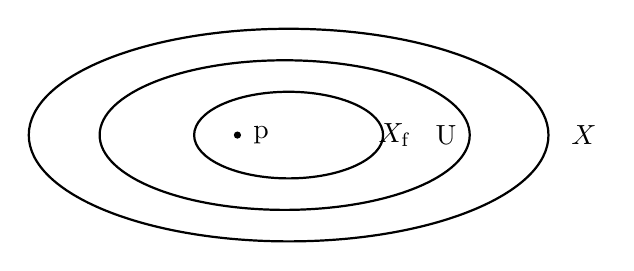
\begin{tikzpicture}[line width=0.8pt]
  \draw (0.2,0) ellipse (3.3 and 1.35);
  \draw (0.15,0) ellipse (2.35 and 0.95);
  \draw (0.2,0) ellipse (1.2 and 0.55);
  \fill (-0.45,0) circle (1.3pt);
  \node[anchor=west] at (-0.38,0) {$\mathrm{p}$};
  \node at (1.55,0) {$X_{\mathrm{f}}$};
  \node at (2.2,0) {$\mathrm{U}$};
  \node at (3.95,0) {$X$};
\end{tikzpicture}
\caption{\mbox{定理~16.2.2} 证明的直观辅助图。（依原书手绘图重绘。）}\label{fig:ample-visual-aid}
\end{figure}

令 $\mathscr{I}$ 为在 $X\setminus\mathrm{U}$ 上消失的那些函数所成的理想层（即以既约结构把 $X\setminus\mathrm{U}$ 割出来的那个\trQC{}理想层）。由于 $X$ 是\trNoether{}的，$\mathscr{I}$ 是\trFiniteType{}的，于是由 $(b)$，对某个 $\mathrm{N}$，$\mathscr{I}\otimes\mathscr{L}^{\otimes\mathrm{N}}$ 由\trGlobalSections{}生成，从而它有一个在 $p$ 处不消失的\trGlobalSections。（\emph{诺特附记}：这是整个论证中唯一用到诺特假设的地方。这些假设可以按如下方式去掉。证明：对一个\trQuasicompact\trQuasiSeparated{}概形，每个理想层都由其\trFiniteType{}的\trSubidealSheaf{}生成。事实上，\trQuasicompact\trQuasiSeparated{}概形上的任何\trQCSheaf{}都是它的\trFiniteType{}的\trQC{}子层之并。这件事可以徒手证明，是一道合用却困难的练习；例如见 [Stacks, tag~01PJ]。这些\trFiniteType{}理想层当中有一个在 $p$ 处不消失；拿它来顶替 $\mathscr{I}$ 即可。）

我们现在不得不开始更卖力地干活了。

我们接着证明 $(c'')$ 蕴含 $(b)$。

我们希望证明：对 $n\gg 0$，$\mathscr{F}\otimes\mathscr{L}^{\otimes n}$ 都是\trGloballyGenerated。我们先来证明 $(c'')$ 蕴含「对某个 $\mathrm{N}>0$，$\mathscr{L}^{\otimes\mathrm{N}}$ 是\trGloballyGenerated」，做法如下。利用 $X$ 的\trQuasicompactness，选出有限多个\trAffine{}的 $X_{\mathrm{f}_1},\dots,X_{\mathrm{f}_n}$ 覆盖 $X$，其中 $\mathrm{f}_i\in\Gamma(X,\mathscr{L}^{\otimes\mathrm{N}_i})$。把 $\mathrm{f}_i$ 换成 $\mathrm{f}_i^{\otimes(\prod_j\mathrm{N}_j)/\mathrm{N}_i}$，便可假定它们都是 $\mathscr{L}$ 的\emph{同一个}幂 $\mathscr{L}^{\otimes\mathrm{N}}$ 的截面（取 $\mathrm{N}=\prod_j\mathrm{N}_j$）。于是 $\mathscr{L}^{\otimes\mathrm{N}}$ 由这些\trGlobalSections{}生成。

我们接着证明：只需对一切\trFiniteType{}的\trQCSheaf{} $\mathscr{F}$ 证明「$\mathscr{F}\otimes\mathscr{L}^{\otimes m\mathrm{N}}$ 在 $m\gg 0$ 时是\trGloballyGenerated」就足够了。因为一旦知道这一点，便可把它施用于 $\mathscr{F}$，$\mathscr{F}\otimes\mathscr{L}^{\vee}$，…，$\mathscr{F}\otimes\mathscr{L}^{\otimes(\mathrm{N}-1)}$（共有限多次），结论随之而来。出于这一理由，我们可以把 $\mathscr{L}$ 换成 $\mathscr{L}^{\otimes\mathrm{N}}$。换言之，为证 $(c'')$ 蕴含 $(b)$，我们还可以添上「$\mathscr{L}$ 是\trGloballyGenerated」这条附加假设。

对每个闭点 $p$，利用 $(c'')$ 选一个形如 $X_{\mathrm{f}}$ 的\trAffine\trOpen\trNeighborhood。于是 $\mathscr{F}|_{X_{\mathrm{f}}}$ 由有限多个\trGlobalSections{}生成（容易的\mbox{练习~16.1.B}——$\Spec A$ 上一个\trFiniteType{}的\trQCSheaf{}对应于一个\trFinitelyGenerated{}的 $A$-\trModule）。由\mbox{练习~15.4.N}，这些生成元中的每一个都可表示成 $\mathscr{F}\otimes\mathscr{L}^{\otimes M(p)}$ 在 $X$ 上的一个\trSection{}除以 $\mathrm{f}^{M(p)}$ 的商。（注意：对每个 $p$，可以取定单独一个 $M(p)$。）于是 $\mathscr{F}\otimes\mathscr{L}^{\otimes M(p)}$ 在 $p$ 处由有限多个\trGlobalSections{}生成。由\mbox{练习~16.1.D}(b)，$\mathscr{F}\otimes\mathscr{L}^{\otimes M(p)}$ 在 $p$ 的某个\trOpen\trNeighborhood{} $\mathrm{U}_p$ 中的所有点处都整体生成。由于 $\mathscr{L}$ 也整体生成，这蕴含：对一切 $M'\ge M(p)$，$\mathscr{F}\otimes\mathscr{L}^{\otimes M'}$ 在 $\mathrm{U}_p$ 的一切点处都整体生成（对照容易的\mbox{练习~16.1.C}）。由 $X$ 的\trQuasicompactness，这些 $\mathrm{U}_p$ 中有限多个便覆盖 $X$，于是（取诸 $M(p)$ 的最大者）证毕。

我们的倒数第二步是证明 $(c'')$ 蕴含 $(a)$。设 $(c'')$ 成立。目标便是找到某个 $\mathscr{L}^{\otimes\mathrm{N}}$ 的若干截面，把 $X$ 嵌入\trProjectiveSpace。选取（拟紧的）$X$ 的一个由 $n$ 个\trAffine\trOpenSubset{}组成的覆盖 $X_{a_1},\dots,X_{a_n}$，其中 $a_1,\dots,a_n$ 都是 $\mathscr{L}$ 的幂的截面。把每个截面换成适当的幂之后，便可假定它们都是 $\mathscr{L}$ 的\emph{同一个}幂（设为 $\mathscr{L}^{\otimes\mathrm{N}}$）的截面。设 $X_{a_i}=\Spec A_i$，其中（利用 $\pi$ 为\trFiniteType{}这一事实）$A_i=A[a_{i_1},\dots,a_{i_j}]/I_i$\footnote{原书此处作「$A_i=\Spec A[a_{i_1},\dots,a_{i_j}]/I_i$」，其中的 $\Spec$ 当系衍文（其前已设 $X_{a_i}=\Spec A_i$，$A_i$ 应为环），径删。——译者注}。由\mbox{练习~15.4.N}，每个 $a_{ij}$ 都形如 $s_{ij}/a_i^{m_{ij}}$，其中 $s_{ij}\in\Gamma(X,\mathscr{L}^{\otimes\mathrm{N}m_{ij}})$（对某个 $m_{ij}$）。令 $m=\max_{i,j}m_{ij}$。于是对每一对 $i,j$，$a_{ij}=(s_{ij}a_i^{m-m_{ij}})/a_i^{m}$。为方便计，令 $b_i=a_i^{m}$，$b_{ij}=s_{ij}a_i^{m-m_{ij}}$；这些都是 $\mathscr{L}^{\otimes m\mathrm{N}}$ 的\trGlobalSections。现在考虑由诸 $b_i$ 与诸 $b_{ij}$ 生成的\trLinearSystem。由于 $\mathrm{D}(b_i)=X_{a_i}$ 覆盖 $X$，这个\trLinearSystem{}是\trBasePointFree{}的，从而（由\mbox{练习~15.2.A}）给出一个到 $\mathbb{P}^{\mathrm{Q}}$ 的\trMorphism（其中 $\mathrm{Q}=\#b_i+\#b_{ij}-1$）。令 $x_1,\dots,x_n,\dots,x_{ij},\dots$ 为 $\mathbb{P}^{\mathrm{Q}}$ 上的射影\trCoordinate（于是 $\mathrm{f}^*x_i=b_i$，而 $\mathrm{f}^*x_{ij}=b_{ij}$）。于是诸\trAffineScheme{}之间的态射 $X_{a_i}\to\mathrm{D}(x_i)$ 都是\trClosedEmbedding，因为相伴的环映射是满射（$A_i$ 的\trGenerator{} $a_{ij}$ 正是 $x_{ij}/x_i$ 的\trImage）。

至此，我们为日后记下这么一件事：我们已经证明了下面这个结论。若 $X\to\Spec A$ 是\trFiniteType{}的，而 $\mathscr{L}$ 满足 $(c'')$，则 $X$ 是到某个\trProjective{} $A$-\trScheme{}的一个\trLocallyClosedEmbedding。（我们没有用到分离性。）我们用\mbox{练习~11.4.C}（「固有的像是固有的」）来断结 $(c'')$ 蕴含 $(a)$ 的证明：这个局部闭嵌入到射影 $A$-概形之中的\trImage{}实际上是闭的，故 $X$ 是一个\trProjective{} $A$-\trScheme。（你可看得出为什么带闭\trImage{}的\trLocallyClosedEmbedding{}实际上是\trClosedEmbedding？）

最后，我们指出 $(a)$ 与 $(b)$ 合起来蕴含 $(a')$：若 $\mathscr{L}^{\otimes\mathrm{N}}$ 是\trVeryAmple{}的（由 $(a)$），而 $\mathscr{L}^{\otimes n}$ 对 $n\ge n_0$ 是\trBasePointFree{}的（由 $(b)$），则由\mbox{练习~16.2.C}，$\mathscr{L}^{\otimes n}$ 对 $n\ge n_0+\mathrm{N}$ 是\trVeryAmple{}的。\hfill$\square$

\textbf{16.2.4.}\ \extrahard\ \emph{\trSemiample\trLineBundle。}\quad 正如一个\trInvertibleSheaf{}在它的某个张量幂是\trVeryAmple{}的时便是\trAmple{}的，若一个\trInvertibleSheaf{} $\mathscr{L}$ 的某个张量幂是\trBasePointFree{}的，我们就称 $\mathscr{L}$ 为\textbf{\trSemiample{}的}（semiample）。（解说：$\mathscr{L}$ 是\trAmple{}的，是说它的某个幂给出一个到\trProjectiveSpace{}的\trClosedEmbedding；$\mathscr{L}$ 是\trSemiample{}的，是说它的某个幂只给出一个到\trProjectiveSpace{}的\emph{\trMorphism}。）我们不会用到这个概念。

\textbf{16.2.5.}\ \hard\ \textbf{绝对情形下的\trAmpleness。}\quad （本节内容日后不会被我们以任何严肃的方式用到。）注意，整体生成已然是一个绝对性的概念，也就是说，它对概形上的一个\trQCSheaf{}有定义，不涉及任何\trMorphism。对\mbox{定理~16.2.2} 的证明稍加检视便知，\trAmpleness{}同样可以在一种绝对的情形下解释。我们把这件事说精确。设 $\mathscr{L}$ 是一个\emph{\trQuasicompact}的概形 $X$ 上的\trInvertibleSheaf。我们称 $\mathscr{L}$ 为\textbf{\trAmple{}的}（ample），若当 $\mathrm{f}$ 跑遍 $\mathscr{L}^{\otimes n}$ 的诸\trSection{}（$n>0$），诸开子集 $X_{\mathrm{f}}=\{p\in X:\mathrm{f}(p)\neq 0\}$ 构成 $X$ 之拓扑的一组\trBase。（我们强调，$X$ 的拟紧性是「$\mathscr{L}$ 是\trAmple{}的」这一条件的一部分。）例如：(i) 若 $X$ 是一个\trAffineScheme，则每个\trInvertibleSheaf{}都是\trAmple{}的；(ii) 若 $X$ 是一个\trProjective{} $A$-\trScheme，则 $\OO(1)$ 是\trAmple{}的。

\textbf{16.2.M.（容易的练习：绝对丰富性的性质）}\quad

（a）取定一个正整数 $n$。证明：$\mathscr{L}$ 是\trAmple{}的，当且仅当 $\mathscr{L}^{\otimes n}$ 是\trAmple{}的。

（b）证明：若 $Z\hookrightarrow X$ 是一个\trClosedEmbedding，而 $\mathscr{L}$ 在 $X$ 上是\trAmple{}的，则 $\mathscr{L}|_Z$ 在 $Z$ 上是\trAmple{}的。

下面这条结果会让你对丰富性的行为方式有几分感觉。我们不会用到它，因而略去其证明（证明见 [Stacks, tag~01Q3]）。不过，该证明的许多部分与\mbox{定理~16.2.2} 中相应的论证如出一辙（或为其推广）。诸陈述的标号编排与\mbox{定理~16.2.2} 中诸陈述的标号编排平行一致。

\textbf{16.2.6.\ \trhTheorem{}（对照\mbox{定理~16.2.2}）。}\ ——\ \emph{设 $\mathscr{L}$ 是一个\trQuasicompact{}概形 $X$ 上的\trInvertibleSheaf。则以下诸条件等价。}

\emph{(b) $X$ 是\trQuasiSeparated{}的，且对每个\trFiniteType{}的\trQCSheaf{} $\mathscr{F}$，存在某个 $n_0$，使得对 $n\ge n_0$，$\mathscr{F}\otimes\mathscr{L}^{\otimes n}$ 都是\trGloballyGenerated。}

\emph{(c) 当 $\mathrm{f}$ 跑遍 $\mathscr{L}^{\otimes n}$ 的诸\trGlobalSections（$n>0$），诸开子集 $X_{\mathrm{f}}=\{p\in X:\mathrm{f}(p)\neq 0\}$ 构成 $X$ 之拓扑的一组\trBase（也就是说，$\mathscr{L}$ 是\trAmple{}的）。}

\emph{(c') 当 $\mathrm{f}$ 跑遍 $\mathscr{L}^{\otimes n}$ 的诸\trGlobalSections（$n>0$），其中\trAffine{}的那些开子集 $X_{\mathrm{f}}$ 构成 $X$ 之拓扑的一组\trBase。}

\emph{(c'') 当 $\mathrm{f}$ 跑遍 $\mathscr{L}^{\otimes n}$ 的诸\trGlobalSections（$n>0$），其中\trAffine{}的那些开子集 $X_{\mathrm{f}}$ 覆盖 $X$。}

\emph{(d) 令 $S_\bullet$ 为分次环 $\oplus_{n\ge 0}\Gamma(X,\mathscr{L}^{\otimes n})$。则诸开集 $X_{\mathrm{f}}$（其中 $\mathrm{f}\in S_+$ 是正次数的\trHomogeneous{}元素）覆盖 $X$，且相伴的映射 $X\to\Proj S_\bullet$ 是一个\trOpenEmbedding。（警告：$S_\bullet$ 未必\trFinitelyGenerated，而 $\Proj S_\bullet$ 也未必是\trFiniteType{}的。）}

$(d)$ 部分蕴含 $X$ 是\trSeparated{}的（从而是\trQuasiSeparated{}的）。

\textbf{16.2.7.}\ \hard\ \textbf{把整体生成、无基点性与丰富性搬运到相对情形。}\quad 这些观念都可以被「相对化」。我们本可以现在就动手做这件事，但我们将等到 \S17.3.5——届时我们将已经定义了\trProjective\trMorphism{}的观念，从而也定义了「相对\trVeryAmple」的\trLineBundle——再做。


\section{曲线上的应用}

现在，我们要把所学应用到\trCurve{}上。（这段讨论之所以来得这么晚，唯一的
原因是：我们需要\mbox{练习~16.2.G}，它蕴含若 $X\to Y$ 是\trFinite{}的，而 $Y$
在 $k$ 上射影，则 $X$ 在 $k$ 上也射影。）由于「\trCurve」一词可以有不同的含义，
我们在定理的陈述中将对假设力求一丝不苟。（在日常用法中，\trCurve{}常指%
\trPureDimension{} $1$ 的、某个\trField{} $k$ 上的\trVariety。）

\textbf{16.3.1.\ 定理（每条整\trCurve{}都有一个正则且射影的双有理模型）。}\ ——\
\emph{若 $C$ 是一个整的、有限型的、一维的 $k$-\trScheme，则存在正则射影的
$k$-\trVariety{} $C'$（维数为 $1$），与 $C$ 双有理。}

\emph{证明。}\quad 我们可以不妨设 $C$ 是\trAffine{}的。由\mbox{\trNoetherNormalization{}引理~12.2.4}，
我们可以找出某个 $x\in K(C)\setminus k$，使 $K(C)/k(x)$ 是一个\trFinite{}的\trFieldExtension。把
$\mathbb{P}^1_k$ 的一个\trStandardOpenSet{}等同于 $\Spec k[x]$，并在\trFunctionField{} $K(C)$
中取 $\mathbb{P}^1_k$ 的\trNormalization（定义见\mbox{练习~10.7.I}），我们便得到一个\trFinite\trMorphism
\[
C'\longrightarrow\mathbb{P}^1_k,
\]
其中 $C'$ 是一条\trCurve（\trFinite{}性由\mbox{练习~10.7.M}，$\dim C'=\dim\mathbb{P}^1_k$
由\mbox{练习~12.1.G}），并且正则（它既约，故在\trGenericPoint{}处正则；而在诸%
\trClosedPoint{}处，正则性由 \S13.5 中关于\trDVR{}的主定理给出）。此外，$C'$ 与 $C$
双有理，因为二者具有同构的\trFunctionField（\mbox{练习~7.5.E}）。

\begin{figure}[htbp]
\centering
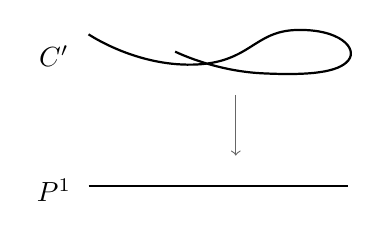
\begin{tikzpicture}[scale=1.1]
  \node at (-0.5,1.5) {$C'$};
  \draw[thick] plot [smooth, tension=1] coordinates {(-0.1,1.75) (1.1,1.4) (2.3,1.8) (2.9,1.45)
    (1.9,1.3) (0.9,1.55)};
  \draw[->, black!60] (1.6,1.05) -- (1.6,0.35);
  \draw[thick] (-0.1,0) -- (2.9,0);
  \node at (-0.5,-0.05) {$\mathbb{P}^1$};
\end{tikzpicture}
\caption{经 $\mathbb{P}^1$ 的一个有限覆盖，构造 $k$ 上\trCurve{} $C$ 的一个射影正则模型。
（依原书手绘图重绘。）}%
\label{fig:curve-proj-regular-model}
\end{figure}

最后，$C'\to\mathbb{P}^1_k$ 是\trFinite{}的，而 $\mathbb{P}^1_k\to\Spec k$ 是射影的，
于是由\mbox{练习~16.2.G}，$C'\to\Spec k$ 是射影的。\hfill$\square$

\textbf{16.3.2.\ 定理。}\ ——\ \emph{若 $C$ 是不可约、正则、一维的 $k$-\trVariety，则存在
一个\trOpenEmbedding{} $C\hookrightarrow C'$，其目标 $C'$ 是某条（$k$ 上的）射影正则\trCurve。}

\emph{证明。}\quad 我们先证 $C$ \trAffine{}的情形。与\mbox{定理~16.3.1} 的证明一样，我们有如下交换图
\[
\begin{tikzcd}[column sep=3.5em, row sep=3.5em]
C \ar[d, "\pi\ \text{有限}"'] & C' \ar[d, "\pi'\ \text{有限}"'] \\
\mathbb{A}^1_k \ar[r, hook] & \mathbb{P}^1_k,
\end{tikzcd}
\]
其中 $\pi'$ 是 $\mathbb{P}^1_k$ 在\trFunctionField{}扩张 $K(C)/K(\mathbb{A}^1_k)$ 中的\trNormalization，而
$C'$ 是射影的。由\trNormalization{}在\trFunctionField{}扩张中的\trUniversalProperty，$\mathbb{A}^1_k$ 在%
\trFunctionField{}扩张 $K(C)/K(\mathbb{A}^1_k)$ 中的\trNormalization{}正是 $C$ 本身，因为 $C$ 已经%
\trNormal。于是 $(\pi')^{-1}(\mathbb{A}^1_k)=C$，这便给出了想要的\trOpenEmbedding{}
$C\to C'$。

接下来我们考虑一般的 $C$。取 $C$ 的任意一个非空\trAffine\trOpenSubset{} $C_1$。由上一段的讨论，
我们有一个正则射影的\textbf{紧化}（compactification）$\widetilde{C}_1$。\mbox{曲线到射影的延拓定理~15.3.1}
（逐次应用于 $C\setminus C_1$ 的有限多个点）蕴含：\trMorphism{} $C_1\hookrightarrow\widetilde{C}_1$
可延拓为一个双有理\trMorphism{} $C\to\widetilde{C}_1$。由于\trSeparated{}正则\trCurve{}的点由其%
\trValuation{}所确定（\mbox{练习~13.7.B}），这便是集合论意义上的包含关系。又因为\trCurve{}上的拓扑是
「\trCofiniteTopology」，它把 $C$ 表为 $\widetilde{C}_1$ 的一个\trOpenSubset。但我们还没有大功告成！
\[
\begin{tikzcd}[column sep=3.5em, row sep=3.2em]
C_1 \ar[dr, hook] \ar[dd] & & \\
& C \ar[dl] & \\
\widetilde{C}_1 & &
\end{tikzcd}
\]
我们尚须证明：$C\to\widetilde{C}_1$ 是概形之间的\emph{\trOpenEmbedding}。为此，我们按如下方式证明它在任一点
$p$ 附近都是\trOpenEmbedding。取 $p$ 在 $C$ 中的一个\trAffine\trOpen\trNeighborhood{} $C_2$。
我们把在 $C_1$ 上用过的构造重演一遍，便得到下面这张标出了诸\trOpenEmbedding{}的交换图
\[
\begin{tikzcd}[column sep=2.8em, row sep=3.8em]
C_1 \ar[dr, hook] \ar[dd] & & C_2 \ar[dl, hook] \ar[dd] \\
& C \ar[dl] \ar[dr] & \\
\widetilde{C}_1 & & \widetilde{C}_2
\end{tikzcd}
\]
由\mbox{曲线到射影的延拓定理~15.3.1}，映射 $C_1\to\widetilde{C}_2$ 可延拓为
$\pi_{12}\colon\widetilde{C}_1\to\widetilde{C}_2$，而类似地我们也有一个\trMorphism{}
$\pi_{21}\colon\widetilde{C}_2\to\widetilde{C}_1$，延拓 $C_2\to\widetilde{C}_1$。复合
$\pi_{21}\circ\pi_{12}$ 是恒等\trMorphism（因为它是恒等\trRationalMap；见\mbox{定理~11.3.2}）。同理
$\pi_{12}\circ\pi_{21}$ 亦然，故 $\pi_{12}$ 与 $\pi_{21}$ 都是\trIsomorphism。于是加料后的交换图
\[
\begin{tikzcd}[column sep=2.8em, row sep=3.8em]
C_1 \ar[dr, hook] \ar[dd] & & C_2 \ar[dl, hook] \ar[dd] \\
& C \ar[dl] \ar[dr] & \\
\widetilde{C}_1 & & \widetilde{C}_2
\ar[ll, "\sim"]
\end{tikzcd}
\]
交换（仍是\mbox{定理~11.3.2}——它蕴含既约分离概形之间的\trMorphism{}由其在\trDense\trOpenSet{}上的
行为所确定）。但 $C_2\to\widetilde{C}_1$ 是一个\trOpenEmbedding（特别是在 $p$ 处），所以
$C\to\widetilde{C}_1$ 在 $p$ 处也是\trOpenEmbedding。\hfill$\square$

\textbf{16.3.A.（练习）}\quad 证明：$k$ 上所有正则的\trProper\trCurve{}都是射影的。

\textbf{16.3.3.\ 定理（\trCurve{}的种种范畴是同一个）。}\ ——\ \emph{以下诸\trCategory{}等价：}

（i）\emph{整的、正则的、射影的一维 $k$-簇，以及满的 $k$-\trMorphism；}

（ii）\emph{整的、正则的、射影的一维 $k$-簇，以及支配的 $k$-\trMorphism；}

（iii）\emph{整的、正则的、射影的一维 $k$-簇，以及支配的 $k$ 上\trRationalMap；}

（iv）\emph{整的、一维的 $k$-簇，以及支配的 $k$ 上\trRationalMap；}以及

（v）\emph{「在 $k$ 上超越次数为 $1$ 的有限生成域，连同 $k$-同态」这一\trCategory{}的%
\trOppositeCategory（定义见 \S1.1.16）。}

在下面的讨论中，一切\trMorphism{}与\trMap{}都默认定义在 $k$ 上。

（旁注：有兴趣的读者可以微调下面的证明，来证明本定理的下述变体。在（i）--（iv）中，只考虑%
\trGeometricallyIrreducible{}的\trCurve；而在（v）中，只考虑满足「在 $\overline{k}$ 中
$K\cap k^s=k$」的域 $K$。这一变体使我们能够排除那些我们未必想考虑的「怪异」\trCurve。例如，
若 $k=\mathbb{R}$，那么我们便允许了诸如 $\mathbb{P}^1_{\mathbb{C}}$ 这类非%
\trGeometricallyIrreducible{}的\trCurve，因为
$\mathbb{P}^1_{\mathbb{C}}\times_{\mathbb{R}}\Spec\mathbb{C}\cong
\mathbb{P}^1_{\mathbb{C}}\amalg\mathbb{P}^1_{\mathbb{C}}$。）

\emph{证明。}\quad 每个满态射都是支配态射，而每个支配态射都是支配有理映射，又每条整的正则射影%
\trCurve{}都是拟射影\trCurve，于是我们已（不严格地说）展示了如何从（i）走到（ii）再走到（iii）
最后走到（iv）。要从（iv）走到（i），设我们有一条整\trCurve{}之间的支配\trRationalMap{}
$C_1\dashrightarrow C_2$。把 $C_1$ 换成一个\trDense\trOpenSet，使该\trRationalMap{}成为一个%
\trMorphism{} $C_1\to C_2$。这诱导出正则不可约\trCurve{}的\trNormalization{}之间的一个映射
$\widetilde{C}_1\to\widetilde{C}_2$。取 $\overline{\widetilde{C}}_i$ 为 $\widetilde{C}_i$ 的一个正则
射影紧化（$i=1,2$），如\mbox{定理~16.3.2} 中那样。于是，由
\mbox{曲线到射影的延拓定理~15.3.1}，\trMorphism{} $\widetilde{C}_1\to\widetilde{C}_2$ 可延拓为%
\trMorphism{} $\overline{\widetilde{C}}_1\to\overline{\widetilde{C}}_2$。这个\trMorphism{}是满的
（你看出缘由了吗？），于是我们便在范畴（i）中造出了一个\trMorphism。

\textbf{16.3.B.（练习）}\quad 把上面的各个部件拼装起来，具体描述范畴（i）至（iv）的等价。

剩下的只是把（v）也接上。这本质上就是\mbox{练习~7.5.E} 的内容；细节留给读者。\hfill$\square$

\mbox{定理~16.3.3} 有好些个推论。例如，每条既约的拟射影\trCurve{}都恰与唯一一条射影正则%
\trCurve{}双有理。下面是另一个有意思的推论。

\textbf{16.3.4.\ 重要观念：从\trCurve{}到正则\trCurve{}的射影态射的次数。}

对于紧致\trRiemann{}曲面之间的映射有一个表现良好的次数——只要以恰当的重数清点原像，$C'$ 的
一个点的原像个数便为常数——你或许已有相当合理的直觉。例如，若 $f$ 局部看起来像
$z\mapsto z^m=y$，那么在 $y=0$ 与 $z=0$ 附近（但不在 $z=0$ 处），每个点都恰有 $m$ 个原像；
而当 $y$ 趋于 $0$ 时，这 $m$ 个原像便并合起来。富有启发性的\mbox{例~10.3.4} 已在一个
更复杂的情境中展示过这个现象。

现在我们来证明这个事实的代数版本。设 $\pi\colon C\to C'$ 是正则射影\trCurve{}之间的一个满
（等价地，支配）映射。我们将证明 $\pi$ 有一个表现良好的次数，其确切含义我们现在就来厘定。

我们先证 $\pi$ 是\trFinite{}的。\mbox{定理~18.1.6}（有限＝射影＋有限\trFiber）蕴含这一点，
但我们还没有证明它。于是，作为替代，我们按如下方式证明 $\pi$ 的\trFinite{}性。取 $C''$ 为
$C'$ 在 $C$ 的\trFunctionField{}中的\trNormalization。那么我们有同构
$K(C)\cong K(C'')$（实际上就是相等），它诱导出双有理映射
$C\mathrel{\leftharpoonup\joinrel\relbar\joinrel\rightharpoondown}C''$；由于 $C$ 与 $C''$ 都
正则且射影，这些映射可延拓为\trMorphism（由\mbox{曲线到射影的延拓定理~15.3.1}）。于是这就给出了
$C$ 与 $C''$ 的一个\trIsomorphism。而由\trNormalization{}的\trFinite{}性
（\mbox{练习~10.7.M}），$C''\to C'$ 是\trFinite\trMorphism。

\textbf{16.3.5.\ 命题。}\ ——\ \emph{设 $\pi\colon C\to C'$ 是一个\trFinite\trMorphism，其中
$C'$ 是\trPureDimension{} $1$ 的正则\trNoetherian\trScheme，而 $C$ 是\trPureDimension{} $1$
且无\trEmbeddedPoint{}的\trNoetherian\trScheme（最重要的情形：$C$ 既约）。那么 $\pi_*\OO_C$
是有限秩的\trLocallyFreeSheaf。}

「无\trEmbeddedPoint」这一假设，等价于要求 $C$ 的每个\trAssociatedPoint{}都映到（$C'$ 的某个
不可约分量的）\trGenericPoint{}上。注意：若 $C$ 既约，则 $C$ 的奇点可以糟糕到什么程度完全不受
限制！

我们将在 \S16.3.11 中证明\mbox{命题~16.3.5}，在那之前先展示它何等有用。$C'$ 上的正则性假设是
必要的：结点曲线（\cref{fig:normalization-nodal-cubic}）的\trNormalization{}便是一例——大多数
点只有一个原像，而有一个点（「\trNode」）却有两个。（在\mbox{注记~24.3.8} 与 \S24.3.12 中我们
将会看到，\mbox{命题~16.3.5} 的诸假设中真正要紧的，是该\trMorphism{}既\trFinite{}又\trFlat。）

\textbf{16.3.6.}\ \emph{\trhDefinition{}。}\quad 若 $C'$ 不可约，则这个\trLocallyFreeSheaf{}的
秩就称为 $\pi$ 的\textbf{\trDegree}。

\textbf{16.3.C.（练习）}\quad 回想：从一条整\trCurve{}到另一条整\trCurve{}的\trRationalMap{}的%
\trDegree{}定义为\trFunctionField{}扩张的\trDegree（\mbox{定义~12.2.2}）。证明：在
\mbox{命题~16.3.5} 的记号下，若 $C$ 与 $C'$ 都是整的，则作为\trRationalMap{}的 $\pi$ 的%
\trDegree{}与 $\pi_*\OO_C$ 的秩相同。

\textbf{16.3.7.}\ \emph{写给具有复解析背景的读者的注记（代数\trDegree{}＝解析\trDegree）。}\quad
若 $C\to C'$ 是正则的复代数\trCurve{}之间的一个\trFinite{}映射，则\mbox{命题~16.3.5} 建立了：
上面定义的代数\trDegree{}与解析\trDegree{}相同（以重数清点原像）。

\textbf{16.3.D.（练习）}\quad 我们沿用\mbox{命题~16.3.5} 的记号与假设。设 $p$ 是 $C'$ 的一个%
\trClosedPoint。$p$ 的概形论原像 $\pi^{-1}(p)$ 是 $k$ 上的一个维数 $0$ 的\trScheme。
（a）设 $C'$ 在某个\trField{} $k$ 上有限型，并设 $n$ 是 $\pi^{-1}(p)$ 的\trStructureSheaf{}的%
\trGlobalSections{}所构成的 $k$-\trVectorSpace{}的\trDimension。证明：
$n=(\deg\pi)(\deg p)$。（点的\trDegree{}定义于 \S5.3.8。）
（b）设 $C$ 正则，并且 $\pi^{-1}(p)=\{p_1,\dots,p_m\}$。设 $t$ 是\trDVR{} $\OO_{C',p}$ 的一个%
\trUniformizer。证明：
\[
\deg\pi=\sum_{i=1}^{m}(\mathrm{val}_{p_i}\,\pi^*t)\,\deg(\kappa(p_i)/\kappa(p)),
\]
其中 $\deg(\kappa(p_i)/\kappa(p))$ 表示剩余域之\trFieldExtension{}的次数。（你能推广（a），把
「在域上工作」的假设去掉吗？如果你是数论工作者，你能用「数域的整数环之扩张中素理想的分裂」的
语言辨认出（b）吗？）

\textbf{16.3.E.（练习）}\quad 设 $C$ 是 $k$ 上一条不可约正则射影\trCurve，而 $s$ 是 $C$ 上的一个非零%
\trRationalFunction。证明：$s$ 的\trZeros{}的个数（以恰当的重数清点）等于其\trPole{}的个数。提示：
把这认作\trMorphism{} $s\colon C\to\mathbb{P}^1_k$ 的次数。对 $0\in\mathbb{P}^1$ 与
$\infty\in\mathbb{P}^1$ 两个情形使用\mbox{练习~16.3.D}(b)。（在复范畴中，这是留数定理的一个重要
推论。）

\textbf{16.3.8.}\ \extrahard\ \emph{一个现在就能作出的重要定义（尽管我们要等到 \S18.4.2）。}\quad
写到这里，我们其实已经能够轻而易举地作出「\trSmooth{}射影\trCurve{}上的\trLineBundle{}的%
\trDegree{}」这一重要定义了。你不妨现在就把它想通，尽管我们要等到 \S18.4.2 才作出一个
（貌似不同的）定义，并在\mbox{重要容易练习~18.4.C} 中证明它与这个定义等价。设 $C$ 是 $k$
上一条不可约正则射影\trCurve，而 $\mathscr{L}$ 是 $C$ 上的一个\trLineBundle。那么
$\mathscr{L}$ 便拥有一个非零\trRational\trSection{} $s$（你看出缘由了吗？）。若 $s$ 与
$t$ 是任意两个非零\trRational\trSection，则由\mbox{练习~16.3.E}，对\trRationalFunction{}
$s/t$ 而言，零点的个数等于极点的个数（正确清点）\footnote{原书此处作「for the the
rational function」，当为「for the rational function」之误，径改。——译者注}。于是，非零%
\trRational\trSection{} $s$ 的「零点个数减去极点个数」（正确清点）不依赖于 $s$ 的选取。
这个整数本可以被取作\trCurve{} $C$ 上\trLineBundle{} $\mathscr{L}$ 的\trDegree{}的定义。
（由于我们并未把它当作「正式定义」，我们就不把这个短语排成粗体。）

\textbf{16.3.9.}\ \emph{\trhRemark{}。}\quad 在\mbox{练习~18.4.E} 中，我们将会看到：上一练习
中零点（与极点）的个数，正是给出到 $\mathbb{P}^1$ 之映射的那个\trLineBundle{}的%
\trDegree（经由\mbox{重要定理~15.2.2}）。

\textbf{16.3.10.}\ \emph{重温\mbox{例~10.3.4}。}\quad \mbox{命题~16.3.5} 与\mbox{练习~16.3.D}
把我们在\mbox{例~10.3.4} 中观察到的一般行为精确化了。设 $C'$ 不可约，并设 $d$ 是这个号称%
\trLocallyFreeSheaf{}的东西的秩。那么，$C'$ 的任一个\trResidueField{}为 $K$ 的点上的%
\trFiber，都是某个 $K$ 上维数为 $d$ 的\trAlgebra{}的 $\Spec$。这意味着\trFiber{}中点的
个数（以恰当的重数清点）总是 $d$。

作为一个动机性的例子，我们重温\mbox{例~10.3.4}：由 $x\mapsto y^2$ 给出的映射
$\mathbb{Q}[y]\to\mathbb{Q}[x]$\footnote{原书此处作「the map $\mathbb{Q}[y]\to\mathbb{Q}[x]$
given by $x\mapsto y^2$」——按「$x\mapsto y^2$」读法，环映射的方向当为
$\mathbb{Q}[x]\to\mathbb{Q}[y]$（\mbox{例~10.3.4} 原文正是如此），此处箭头疑当为笔误，
兹照录原书。——译者注}，即\trParabola{} $x=y^2$ 到 $x$-轴的\trProjection。我们当时观察到
如下现象。
（i）$x=1$ 之上的\trFiber{}是 $\mathbb{Q}[y]/(y^2-1)$，于是我们得到 $2$ 个点。
（ii）$x=0$ 之上的\trFiber{}是 $\mathbb{Q}[y]/(y^2)$——我们得到一个点，重数为 $2$，
起因于非既约性。
（iii）$x=-1$ 之上的\trFiber{}是 $\mathbb{Q}[y]/(y^2+1)\cong\mathbb{Q}(i)$——我们得到一个
点，重数为 $2$，起因于\trFieldExtension。
（iv）最后，\trGenericPoint{} $\Spec\mathbb{Q}(x)$ 之上的\trFiber{}是 $\Spec\mathbb{Q}(y)$，
这是一个点，重数为 $2$，同样起因于\trFieldExtension（因为 $\mathbb{Q}(y)/\mathbb{Q}(x)$
是 $2$ 次的\trFieldExtension）。
于是我们看到三种行为（其中情形（iii）与（iv）实为同一回事）。注意：即便你只在%
\trAlgClosedField{}上工作，你仍然会被迫去对付这第三种行为，因为\trGenericPoint{}处的%
\trResidueField{}通常不\trAlgClosed（上面的情形（iv）便是明证）。

\textbf{16.3.11.}\ \emph{\mbox{命题~16.3.5} 的证明。}\quad 其中的关键想法——它在别的场合也有
用——是化归到关于\trDVR{}的一个事实。

这个问题在靶上是局部的，故不妨设 $C'$ 是\trAffine{}的。如今 $C'$ 是\trNormal{}的，于是由
\mbox{练习~5.4.B}，它的诸\trConnectedComponent{}都不可约。把 $C'$ 换成它的每一个%
\trIrreducibleComponent，我们还不妨设 $C'$ 是整的。

由\mbox{练习~14.3.K}，若有限型\trQCSheaf{} $\pi_*\OO_C$ 的秩是常数，则（由于 $C'$ 既约）
$\pi_*\OO_C$ 是\trLocallyFree{}的。我们将这样来证明它：证明 $C'$ 在任一\trClosedPoint{} $p$
处的秩与它在\trGenericPoint{}处的秩相同。（这是\trGenericPoint{}之有用性的又一个例子。）

设 $C'=\Spec A'$，其中 $A'$ 是一个\trIntegralDomain，并设 $p=[\mathfrak{m}]$。由于 $\pi$
是\trAffine\trMorphism，$C$ 也是\trAffine\trScheme；比如说，$C=\Spec A$。

我们希望证明：（i）$\dim_{A'/\mathfrak{m}}(A/\mathfrak{m})$（$\pi_*\OO_C$ 在 $p$ 处的秩）
等于（ii）$\dim_{K(A')}(A'^\times)^{-1}A$（$\pi_*\OO_C$ 在\trGenericPoint{}处的秩）。换个
话说，我们取 $A$（视作一个 $A'$-\trModule），然后（i）模掉 $\mathfrak{m}$，（ii）把 $A'$
的全部非零元都取逆，再在每种情形下计算所得者在相应\trField{}上的维数。

（i）与（ii）都穿过在 $\mathfrak{m}$ 处的\trLocalization{}分解，故只需证明：
$A_{\mathfrak{m}}$ 是一个秩有限的自由 $A'_{\mathfrak{m}}$-\trModule，比如说秩为 $d$——
因为届时（i）与（ii）的答案都将是 $d$。

如今 $A'_{\mathfrak{m}}$ 是一个\trDVR；设 $t$ 是它的\trUniformizer。我们可以假设
$t\in A'$（因为不然的话，我们就把 $A'$ 换成一个适当的\trLocalization，即在 $t$ 的诸
「分母」处取局部化）。此时 $A_{\mathfrak{m}}$ 是有限生成的 $A'_{\mathfrak{m}}$-\trModule，
从而由\mbox{注记~6.4.4}，它是\trPrincipalModule（principal module）的有限\trDirectSum，形状为 $A'_{\mathfrak{m}}$
或 $A'_{\mathfrak{m}}/(t^n)$（$n$ 取各种值）。我们希望证明：后一类型的直和项并不出现。
但倘若出现，则 $t$（解释为 $A_{\mathfrak{m}}$ 中的元素）将是 $A_{\mathfrak{m}}$ 的一个%
\trZerodivisor，从而（解释为 $A$ 中的元素）是 $A$ 的\trZerodivisor。但那样一来，由
\mbox{命题~6.6.13}，在 $\pi^{-1}(p)$ 中便有 $C$ 的一个\trAssociatedPoint，这与「$C$
无\trEmbeddedPoint」的假设相矛盾。\hfill$\square$



\section{\hard\ \trGrassmannian{}作为\trModuliSpace}

（在本节及其他几节中，记号 $k$ 既用作一个\trField，也用作一个维数。对此我们深表歉意，希望它不至于引起太大的混淆。）

我们最初在 \S4.4.9 中以不大体面的方式定义了\trProjectiveSpace，而在 \S15.2.3 中给出了一个干净（尽管也许出人意料）的\trFunctor{}式定义。类似地，我们在 \S7.7 中给出了\trGrassmannian{}的一份初步描述。如今我们已有条件给出一个更好的定义。在继续之前，如果你还没有读过 \extrahard{}节 \S10.1.7，应当先回头去读一读。

我们来描述「\trGrassmannian{}（\trContravariantFunctor）」（我们也把它记作 $\mathrm{G}(k,n)$），然后证明它是\trRepresentable{}的（\S7.6.2）。这一构造在任意\trBaseScheme{}上都行得通，于是我们在\trFinalObject{} $\Spec\mathbb{Z}$ 上工作。（倘若你想在比如复概形上工作，应当先想清楚要改动些什么。）这个\trFunctor{}定义如下。对一个\trScheme{} $B$，我们给它配上由秩 $n$ 自由层的\emph{局部自由秩 $k$ 商}
\begin{equation*}\tag{16.4.0.1}\label{eq:grassmannian-rank-k-quotient}
\OO_{\mathrm{B}}^{\oplus n}\twoheadrightarrow\scr{Q},
\end{equation*}
（\emph{不计\trIsomorphism}）所构成的集合。两个这样的商 $\phi\colon\OO_{\mathrm{B}}^{\oplus n}\to\scr{Q}\to 0$ 与 $\phi'\colon\OO_{\mathrm{B}}^{\oplus n}\to\scr{Q}'\to 0$ 之间的一个\trIsomorphism，是指一个\trIsomorphism{} $\sigma\colon\scr{Q}\overset{\sim}{\longrightarrow}\scr{Q}'$，它使下图交换：
\[
\begin{tikzcd}
\OO^{\oplus n} \ar[r, "\phi"] \ar[dr, "\phi'"'] & \scr{Q} \ar[d, "\sigma"] \\
& \scr{Q}'
\end{tikzcd}
\]
由\mbox{练习~14.2.H}(a)，$\ker\phi$ 是秩 $n-k$ 的\trLocallyFreeSheaf。（于是，如果你愿意，可以将 \eqref{eq:grassmannian-rank-k-quotient} 扩充，转而让这个\trFunctor{}把 $B$ 送到 $B$ 上\trLocallyFreeSheaf{}的如下\trShortExactSequence
\begin{equation*}\tag{16.4.0.2}\label{eq:grassmannian-tautological-ses}
0\longrightarrow\scr{S}\longrightarrow\OO^{\oplus n}\longrightarrow\scr{Q}\longrightarrow 0
\end{equation*}
其秩分别为 $n-k$、$n$、$k$。）

看到这里你也许会吃惊：格拉斯曼本应参数化 $n$ 维空间中的 $k$ 维\trSubspace{}\footnote{原书此处作「k-dimensional subspace」，subspace 为单数，疑当为复数 subspaces，兹照录原书。——译者注}，而我们考虑的却是秩 $n$ 层的秩 $k$ \emph{商}，而非秩 $k$ \emph{\trSubobject}。这样做有好几个理由。其一是，\trLocallyFreeSheaf{}之间的满射的\trKernel{}必是\trLocallyFreeSheaf，而\trLocallyFreeSheaf{}之间的单射的\trCokernel{}却未必是\trLocallyFreeSheaf{}（分别见\mbox{练习~14.2.H}(a) 与 (b)）。（如果你愿意，也可以不考虑有限秩\trLocallyFreeSheaf{}的满射，而是等价地考虑有限秩\trLocallyFreeSheaf{}的单射——按\mbox{定义~14.2.4} 的说法，即「\trVectorBundle{}的单射」。）理由之二是：在 \S25.3.3 中我们将会看到，这个问题的几何化身确实恰好翻译成了这种提法。在这里我们已然能看到一个关键例子：若 $k=1$，我们的定义给出的便是一维商 $\OO^{\oplus n}\to\scr{L}\to 0$。而这恰好就是「$\scr{L}$ 的 $n$ 个没有公共零点的\trSection{}」这份数据；由\mbox{定理~15.2.2}（\trProjectiveSpace{}的\trFunctor{}式描述），它恰好对应于到 $\mathbb{P}^{n-1}$ 的映射，所以 $k=1$ 的情形参数化的正是我们想要的东西。

现在我们来证明：对给定的 $n$ 与 $k$，\trGrassmannian{}（\trContravariantFunctor）是\trRepresentable{}的。

到目前为止，我们描述了\trGrassmannian{}\trFunctor{}在\emph{\trObject} $B$ 上做什么；而要完整地描述一个\trFunctor，我们还得说明它在\emph{\trMorphism} $B_1\to B_2$ 上做什么。你能看出这个定义必然是什么吗？

\textbf{16.4.A.（练习）}\quad 证明：\trGrassmannian{}\trFunctor{}是一个\trZariskiSheaf（\S10.1.8）。

于是，由\mbox{关键练习~10.1.H}，要证明\trGrassmannian{}\trFunctor{}是\trRepresentable{}的，我们只消用\trRepresentable{}的\trOpen\trSubfunctor{}覆盖它即可。

在本节余下的部分里，一个\textbf{$k$-子集}（$k$-subset）就是 $\{1,\dots,n\}$ 的一个大小为 $k$ 的子集。

\textbf{16.4.B.（练习）}

（a）设 $I$ 是一个 $k$-子集。把下面的陈述说精确：存在\trOpen\trSubfunctor{} $\mathrm{G}(k,n)_I\subset\mathrm{G}(k,n)$，使得 $\scr{Q}$ 的对应于 $I$ 的那 $k$ 个\trSection{}（在来自满射 $\phi\colon\OO^{\oplus n}\to\scr{Q}$ 的 $\scr{Q}$ 的 $n$ 个\trSection{}之中）是线性无关的。提示：在 $\scr{Q}$ 的一个\trTrivialization{}开邻域上，我们可以选取\trIsomorphism{} $\scr{Q}\overset{\sim}{\longrightarrow}\OO^{\oplus k}$，于是 $\phi$ 可被解读为一个 $k\times n$ 矩阵 $M$，而这个轨迹就是 $M$ 的由 $I$ 给出的那些列所拼成的 $k\times k$ 矩阵的\trDeterminant{}可逆的轨迹。证明这个轨迹在平凡化的转换下表现良好。

（b）证明：当 $I$ 取遍全部 $k$-子集时，这些\trOpen\trSubfunctor{} $\mathrm{G}(k,n)_I$ 覆盖\trFunctor{} $\mathrm{G}(k,n)$。

于是，由\mbox{练习~10.1.H}，要证明 $\mathrm{G}(k,n)$ 是\trRepresentable{}的，我们只消证明：$\mathrm{G}(k,n)_I$ 对任意的 $I$ 都是\trRepresentable{}的。把 $\OO^{\oplus n}$ 的各个直和项重新命名之后，不失一般性可设 $I=\{1,\dots,k\}$。

\textbf{16.4.C.（练习）}\quad 证明：$\mathrm{G}(k,n)_{\{1\ldots,k\}}$\footnote{原书此处下标作「$\{1\ldots,k\}$」，「1」之后疑脱一逗号，兹照录原书。——译者注}由 $\mathbb{A}^{k(n-k)}$ 按如下方式表示。（你必须把它说精确。）给定一个满射 $\phi\colon\OO^{\oplus n}\to\scr{Q}$，令 $\phi_i\colon\OO\to\scr{Q}$ 为来自 $\OO^{\oplus n}$ 第 $i$ 个直和项的映射。（\emph{说实话}，$\phi_i$ 只不过是 $\scr{Q}$ 的一个\trSection{}。）对于\trOpen\trSubfunctor{} $\mathrm{G}(k,n)_I$，证明
\[
\phi_1\oplus\cdots\oplus\phi_k\colon\OO^{\oplus k}\longrightarrow\scr{Q}
\]
是一个\trIsomorphism。对一个\trScheme{} $B$，双射 $\mathrm{G}(k,n)_I(B)\leftrightarrow\Hom(B,\mathbb{A}^{k(n-k)})$ 给定如下。给定一个元素 $\phi\in\mathrm{G}(k,n)_I(B)$，对 $j\in\{k+1,\dots,n\}$，有 $\phi_j=a_{1j}\phi_1+a_{2j}\phi_2+\cdots+a_{kj}\phi_k$，其中诸 $a_{ij}$ 都是 $B$ 上的函数。但 $B$ 上的 $k(n-k)$ 个函数与一个到 $\mathbb{A}^{k(n-k)}$ 的映射是一回事（\mbox{练习~7.6.E}）。反之，给定 $k(n-k)$ 个函数 $a_{ij}$（$1\le i\le k<j\le n$），如下定义一个满射 $\phi\colon\OO^{\oplus n}\to\OO^{\oplus k}$：$(\phi_1,\dots,\phi_k)$ 是恒同映射，而对 $j>k$，$\phi_j=a_{1j}\phi_1+a_{2j}\phi_2+\cdots+a_{kj}\phi_k$。

这样，你已经用 $\binom{n}{k}$ 份 $\mathbb{A}^{k(n-k)}$ 覆盖了 $\mathrm{G}(k,n)$，从而证明了它是\trRepresentable{}的。（你或许愿意把这件事与你在 \S7.7 中给出的描述联系起来。）特别地，域上的\trGrassmannian{}是\trSmooth{}的，并且是\trIrreducible{}的，其维数为 $k(n-k)$。（任何基上的\trGrassmannian{}都在该基上\trSmooth，因为 $\mathbb{A}_{\mathrm{B}}^{k(n-k)}\to B$ 是\trSmooth{}的；见 \S13.6.2。）

\textbf{16.4.1.}\ \emph{\trGrassmannian{}上的\trUniversalExactSequence。}\quad 注意，我们有一条重言正合列
\[
0\longrightarrow\scr{S}\longrightarrow\OO^{\oplus n}\longrightarrow\scr{Q}\longrightarrow 0.
\]
丛 $\scr{Q}$ 被称作\trGrassmannian{}上的\textbf{\trTautologicalQuotientBundle}（tautological quotient bundle），而 $\scr{S}$ 被称作\textbf{\trTautologicalSubbundle}（tautological subbundle）。（\mbox{练习~1.2.Z}(b) 或许能让你约略领会，它为何可以称作「\trUniversalExactSequence」（universal exact sequence）。）

\textbf{16.4.2.\ \trPluckerEmbedding。}

对一个满射 $\phi\colon\OO^{\oplus n}\to\scr{Q}$（在任意基 $B$ 上）施加 $\wedge^k$，我们便得到一个满射
\[
\wedge^k\phi\colon\OO^{\oplus\binom{n}{k}}\longrightarrow\det\scr{Q}
\]
（\mbox{练习~14.2.N}）。但从秩 $N$ 自由层出发到一个\trLineBundle{}的满射，与一个到 $\mathbb{P}^{N-1}$ 的映射是同一回事（\mbox{定理~15.2.2}）。

\textbf{16.4.D.（练习）}\quad 利用这一点描述一个映射 $P\colon\mathrm{G}(k,n)\to\mathbb{P}^{\binom{n}{k}-1}$。（这只是一个同义反复：\trFunctor{}之间的一个\trNaturalTransformation{}诱导出表示它们的概形之间的一个映射。这正是\trYonedaLemma，不过，如果你没做过\mbox{练习~1.2.Z}，你也许愿意亲手做一做这个练习。但一旦做了，你也不妨回头去证明\trYonedaLemma{}，再做一做\mbox{练习~1.2.Z}，因为论证完全是一回事！）

\textbf{16.4.E.（练习）}\quad $\mathbb{P}^{\binom{n}{k}-1}$ 上对应于 $\OO^{\oplus\binom{n}{k}}$ 第 $I$ 个直和项的射影\trCoordinate{} $\mathrm{x}_I$，可以解读为映射 $\phi_I\colon\OO^{\oplus k}\to\scr{Q}$ 的\trDeterminant，其中这个 $\OO^{\oplus k}$ 由 $\OO^{\oplus n}$ 中对应于 $I$ 的那些直和项构成。请把这件事说精确。

\textbf{16.4.F.（练习）}\quad 证明：$\mathbb{P}^{\binom{n}{k}-1}$ 中对应于 $k$-子集 $I$ 的\trStandardOpenSet{} $\mathrm{U}_I$（也就是对应的\trCoordinate{} $\mathrm{x}_I$ 不消失之处）拉回正是\trOpen\trSubscheme{} $\mathrm{G}(k,n)_I\subset\mathrm{G}(k,n)$。记这个映射为 $P_I\colon\mathrm{G}(k,n)_I\to\mathrm{U}_I$。

\textbf{16.4.G.（练习）}\quad 证明：$P_I$ 是一个\trClosedEmbedding，做法如下。我们可以只处理 $I=\{1,\dots,k\}$ 的情形。注意 $\mathrm{G}(k,n)_I$ 是仿射的——你在\mbox{练习~16.4.C} 中已经描述了 $\Spec\mathbb{Z}[a_{ij}]_{1\le i\le k<j\le n}$\footnote{原书此处作「you described it Spec $\mathbb{Z}[a_{ij}]$」，当为「described it as Spec $\mathbb{Z}[a_{ij}]$」之脱漏，译文径顺化。——译者注}。此外，$\mathrm{U}_I$ 也是仿射的：当 $I'$ 取遍其余 $k$-子集时，它以诸 $\mathrm{x}_{I'/I}$ 为\trCoordinate。（$k=1$ 的情形，正是我们用来命名\trProjectiveSpace{}各卡上\trCoordinate{}的那个有用记号 $\mathrm{x}_{i/j}$，见 \S4.4.9。）你想证明映射
\[
P_I^{\sharp}\colon\mathbb{Z}[\mathrm{x}_{I'/I}]_{I'\subset\{1,\dots,n\},\,|I'|=k}/(\mathrm{x}_{I/I}-1)\longrightarrow\mathbb{Z}[a_{ij}]_{1\le i\le k<j\le n}
\]
是满射。\footnote{原书此展示式下标中「$|I'|=k$」之后衍一右花括号，径删。——译者注}把映射 $\phi\colon\OO^{\oplus n}\to\OO^{\oplus k}$ 解读为一个 $k\times n$ 矩阵 $M$——其左边 $k$ 列是单位矩阵，而其余元素是 $a_{ij}$（$1\le i\le k<j\le n$）——据此把 $P_I^{\sharp}$ 解读为把 $\mathrm{x}_{I'/I}$ 送到与 $I'$ 中那些列相对应的 $k\times k$ 子矩阵的\trDeterminant。对每一对 $(i,j)$（其中 $1\le i\le k<j\le n$），找出某个 $I'$ 使得 $\mathrm{x}_{I'/I}\mapsto\pm a_{ij}$。（取 $I'=\{1,\dots,i-1,i+1,\dots,k,j\}$。）

于是 $\mathrm{G}(k,n)\to\mathbb{P}^{\binom{n}{k}-1}$ 是一个\trClosedEmbedding，故 $\mathrm{G}(k,n)$ 在 $\mathbb{Z}$ 上是射影的。

\textbf{16.4.H.（不重要的练习）}\quad 一个有趣的几何推论：设 $V$ 是一个域上的\trVectorSpace，证明「$\wedge^k V$ 中的\trPureTensor{}恰以唯一的一种方式为纯」：若在 $\wedge^k V$ 中 $v_1\wedge\cdots\wedge v_k=w_1\wedge\cdots\wedge w_k\neq 0$，证明存在一个\trDeterminant{}为 $1$ 的 $k\times k$ 矩阵，把诸 $v_i$ 与诸 $w_i$ 联系起来。

\textbf{16.4.3.}\ \emph{\trPlucker{}方程。}\quad $\mathrm{G}(k,n)\to\mathbb{P}^{\binom{n}{k}-1}$ 的方程格外好看。在一个 $k\times n$ 矩阵\footnote{原书此处作「k × (n−k) 矩阵」，当为「k × n 矩阵」之误——普吕克坐标正是 $k\times n$ 矩阵的各 $k\times k$ \trMinor，本节\mbox{练习~16.4.B} 与\mbox{练习~16.4.G} 中亦是如此——径改。——译者注}的诸 $k\times k$ \trMinor{}之间存在一些二次关系，称作\trPlucker{}方程。按我们的构造，它们是 $\mathrm{G}(k,n)$ 所满足的方程。事实证明，这些方程恰好切出 $\mathrm{G}(k,n)$，而且实际上生成 $\mathrm{G}(k,n)$ 的\trHomogeneous\trIdeal，不过这要费更多功夫（见 [F1, \S9.1, Lem.~1]）。我们在一个例子中对它作一番探讨。

\textbf{16.4.I.（练习）}\quad 设 $v_1$、$v_2$、$v_3$、$v_4$ 是某个域上一个二维\trVectorSpace{} $V$ 中的四个向量。证明
\[
(v_1\wedge v_2)(v_3\wedge v_4)-(v_1\wedge v_3)(v_2\wedge v_4)+(v_1\wedge v_4)(v_2\wedge v_3)=0.
\]
这个练习的棘手之处在于弄清楚如何解读此处的乘法（诸\trPlucker{}坐标的乘法）。

\textbf{16.4.J.（练习）}\quad 注意，\trPluckerEmbedding{}把\trGrassmannian{} $\mathrm{G}(2,4)$ 嵌入 $\mathbb{P}^5$。

（a）证明：$\mathrm{G}(2,4)$ 由二次方程
\[
\mathrm{x}_{12}\mathrm{x}_{34}-\mathrm{x}_{13}\mathrm{x}_{24}+\mathrm{x}_{14}\mathrm{x}_{23}=0.
\]
切出。（提示：利用\mbox{练习~16.4.I} 证明这个二次式在 $\mathrm{G}(2,4)$ 上消失。但仅止于此还不够。）

（b）证明：特征不为 $2$ 的\trAlgClosedField{} $\overline{k}$ 上，$\mathbb{P}^5$ 中的每一张\trSmooth{}\trQuadricHypersurface{}都\trIsomorphic{}于\trGrassmannian{}（在 $\overline{k}$ 上）。（作为比较：$\mathbb{P}^1_k$ 中的每张\trSmooth{}\trQuadricHypersurface{}是两个点；$\mathbb{P}^2_k$ 中的每张\trSmooth{}\trQuadricHypersurface\trIsomorphic{}于 $\mathbb{P}^1_k$，\S7.5.10；而 $\mathbb{P}^3_k$ 中的每张\trSmooth{}\trQuadricHypersurface\trIsomorphic{}于 $\mathbb{P}^1_k\times_{\overline{k}}\mathbb{P}^1_k$，\mbox{例~10.6.2}。）

\textbf{16.4.K.（练习：$\mathbb{P}^5$ 中\trQuadricSurface{}上的\trRuling）}\quad 设 $k=\overline{k}$。由\mbox{注记~9.3.10}，我们预期 $\mathrm{G}(2,4)$（经由\trPluckerEmbedding{}把它视作 $\mathbb{P}^5$ 中的一张超曲面；见\mbox{练习~16.4.I}）中有两个由平面组成的三维族。其中一族可以描述如下：对每一点 $p\in\mathbb{P}^3_k$，我们有一族过 $p$ 的直线，它是二维的；这就给出 $\mathrm{G}(2,4)$ 中的一个平面。随 $p$ 的不同选取，这些平面构成一个三维的族。这是两条\trRuling{}中的一条。另一条是什么？证明（就你所掌握的内容，能证得多严格就证得多严格）这两者确实都是\trRuling。

\textbf{16.4.4.}\ \emph{进一步的讨论。}

\textbf{16.4.L.（练习）}\quad 证明：\trGroupScheme{} $\mathrm{GL}_n$ 作用在\trGrassmannian{} $\mathrm{G}(k,n)$ 上。（\trGroupScheme{}的\emph{作用}早先出现在\mbox{练习~7.6.S}(a) 中。）提示：用\trFunctor{}的语言（\S7.6）来做这件事，比用开片来描述\trGrassmannian{}（\S7.7）要容易得多。（\mbox{练习~15.5.F} 曾是\trProjectiveSpace{}的特殊情形。）

\textbf{16.4.M.}\ \extrahard\ （练习：\trGrassmannianBundle）\quad 设 $\scr{F}$ 是一个概形 $X$ 上秩为 $n$ 的\trLocallyFreeSheaf。定义 $X$ 上的\textbf{\trGrassmannianBundle}（Grassmannian bundle）$\mathrm{G}(k,\scr{F})$。直观地说，若 $\scr{F}$ 是 $X$ 上 $n$ 维\trVectorSpace{}的一个变动的族，则 $\mathrm{G}(k,\scr{F})$ 应当参数化各\trFiber{}的 $k$ 维商。你不妨先定义这个\trFunctor，然后证明它是\trRepresentable{}的。你的构造在\trBaseChange{}之下将表现良好。

\textbf{16.4.5.}\ \emph{（部分）\trFlagVariety。}\quad 这里的讨论可以原封不动地推广到\trPartialFlagVariety（\S7.7.1），有兴趣的读者应当把这件事想清楚。

